\FrontmatterChapter{Resumen}
{\setlength{\parindent}{0pt}
\begin{Large}
\textbf{SISTEMA DE VISIÓN ARTIFICIAL BASADO EN UN DATASET SINTÉTICO PARA UNA APLICACIÓN DE PICK AND PLACE}
\end{Large}

\textbf{Autor: Ortiz de Zúñiga Mingot, Ignacio.} \\
Director: Jesús López López, Álvaro \& Rodrigo Tobías, Ignacio de \\
Entidad colaboradora: Grupo Antolin \\

\section*{Introducción}
El fin de este proyecto es la generación de un nuevo sistema de visión artificial para el reconocimiento de piezas de uso industrial. Este sistema se implantará dentro de una cadena de suministro del Grupo Antolín\textsuperscript{\textregistered} que a su vez alimentará a una linea de montaje y ensamblaje. El sistema deberá de poder identificar múltiples piezas y determinar el punto de agarre óptimo de cada pieza. Este se ve definido por sus coordenadas así como el vector normal a la superficie. De esta forma un brazo robótico con un sistema de agarre por aspiración, ventosa o \textit{soft-robotics} (varía en función de la pieza a coger) podrá recolectarlas. La multitud de herramientas de agarre así como de la necesidad de un sistema de determinación de puntos de agarre se debe a la gran variedad de piezas existentes con formas y tamaños de gran variedad (1-30 cm).\\
\textbf{Palabras clave:} Visión artificial, Redes neuronales, Regressor, YOLO, Robótica, Linea de ensamblado

\section*{1. Definición del proyecto}
El objetivo del proyecto en colaboración con el grupo Antolin es la creación de un sistema capaz de automatizar el proceso de elaboración de pedidos. El sistema estará constituido por sistemas de visión y brazos robóticos encargados de elaborar "cestas" con todas las piezas necesarias para montar un pedido el cual será ensamblado por un operario. Gracias a la automatización de la generación de las "cestas" se espera poder reducir el tiempo necesario para la elaboración de los pedidos mejorando así la eficiencia del proceso. El proceso completo se puede dividir en varias etapas:

\begin{enumerate}
\item Generación del pedido: en función de la demanda y de los requisitos del cliente se debe de generar una lista con todos los componentes necesarios para cada pedido.
\item Estructuración del pedido: Las piezas necesarias se encuentran distribuidas en diferentes secciones y es por ello que se debe de crear un  que determine el orden de recolección de piezas optimo que reduzca el tiempo recolección.
\item Recolección de piezas: Se trata de un proceso iterativo que se debe de realizar para cada una de las piezas que constituyen el pedido.
\begin{enumerate}[label*=\arabic*.]
\item Desplazamiento hasta la pieza. Dependiendo de la configuración del robot este sistema variará, pero el objetivo siempre será el mismo. Trasladar el robot hasta la región donde se encuentra la pieza a recolectar con el fin de poder capturarla y situarla dentro de la región de alcance.
\item Detección de la pieza: aplicando algoritmos de detección se identificará la pieza que se desea recolectar. Dentro de una misma zona se detectarán numerosas instancias de una misma pieza. Se debe de escoger la pieza/piezas mejor ubicadas y con más probabilidad de éxito.
\item Punto de agarre: tras detectar la pieza se debe de determinar como se debe de agarrar la pieza. Para ello se debe de determinar el punto de agarre óptimo y el vector normal a dicho.
\item Recolección de la pieza: se transfiere la información necesaria al robot para que este pueda recolectar la pieza a través del punto de agarre definido. El sistema de agarre a emplear dependerá del tpo de pieza.
\item Deposición y control de calidad: por último se debe de depositar la pieza dentro de la cesta que constituye el pedido. Y mediante el sistema de visión artificial se debe de comprobar que la pieza deseada ha sido correctamente depositada en la cesta.
\end{enumerate}
\item Control de calidad y trazabilidad: antes de dar por finalizado en pedido se analiza por última vez para comprobar que todas las piezas necesarias se encuentran dentro de la cesta. Se registra en el sistema el pedido y toda la información necesaria para futura trazabilidad.
\item Traslado del pedido: una vez se da por finalizado el pedido este se debe de trasladar hasta la zona de ensamblaje para comenzar el proceso de montado.
\end{enumerate}

En este proyecto nos centraremos unicamente en el desarrollo de una herramienta/sistema de visión artificial que permitirá la detección de la pieza así como la definición del punto de agarre y el vector normal a este. Este sistema se implantará para llevar a cabo la etapa 3.2 así como 3.3. El sistema también puede ser usado en las etapas 3.5 y 4 para llevar acabo las tareas de control de calidad y trazabilidad.

El sistema estará constituido por dos elementos que trabajarán en armonía. Un generador de imágenes capaz crear imágenes de las piezas en un entorno de trabajo así como de obtener la información necesaria de la posición de cada pieza, los puntos de agarre y sus vectores de agarre. Y un sistema de visión artificial basada en redes convolucionales y un regresor para la predicción del punto de agarre óptimo de cada pieza.

\section*{2. Descripción del sistema}
Debido a la necesidad de establecer el punto de agarre óptimo a cada pieza el sistema debe de crecer en complejidad lo cual implica que el \textit{dataset} empleado debe de hacerlo en la misma medida. Se desea tener para cada pieza un elevado número de imágenes con las que poder entrenar tanto a YOLO como a TINY YOLO. Pero además, se desea saber para cada una de las regiones marcadas para TINY YOLO se debe de saber las coordenadas del punto de agarre y su vector normal. Extraer esta información de forma manual es un proceso complejo y con un coste de tiempo elevado. Sobretodo si se considera que idealmente se debe de obtener miles de instancias de cada pieza para entrenar las redes neuronales.

Por este motivo se ha optado por emplear un generador de imágenes basado en la herramienta de renderizado Blender y en la extensión BlenderProc. La extensión es un \textit{pipeline} desarrollado por DLR-RM con el fin simplificar el proceso de generación de \textit{datasets} de imágenes para entrenar redes convolucionales \citep{denninger2019blenderproc}. Se caracteriza por centrarse en la modularidad al dotar a blender con las herramientas necesarias para generar escenas fotorealistas y de forma aleatoria pero manteniendo una estructura modular que permite adaptarse al problema.

Con la ayuda de BlenderProc se ha creado un sistema de generación de imágenes basado en dos partes. En una primera instancia se genera dos escenas idénticas salvo por la excepción de las piezas usadas. En la primera imagen se muestra cada una de las piezas con sus texturas originales. En la segunda se emplea una pieza con una textura modificada con la inserción de códigos QR que más adelante se emplearán para extraer la información restante. A continuación, se muestro el proceso de generación de imágenes:

\begin{enumerate}
\item Escena: Carga del entorno, de las piezas, la iluminación y la cámara. Durante todo este proceso se han empleado motores de aleatoriedad de forma que el escenario, el tipo de piezas y el número de piezas cargadas sea aleatorio. Por último, se carga la cámara y se fijan sus hiperparámetros con el fin de asemejarla a la cámara empleada durante las pruebas.

\item Simulación: activación de las piezas de forma que pasen a formar parte de la simulación y puedan interactuar con el entorno, posicionamiento aleatorio de las piezas y simulación física. De esta forma se consigue crear escenarios aleatorios donde las piezas siempre se encuentran en posiciones realistas y dentro de la zona de trabajo.

\item Renderizado: configuración de los motores de renderizado y escritura de la salida de blender. La configuración empleada en este proceso dependerá del tipo de pieza presente en la escena.
\end{enumerate}

Una vez se ha generado el conjunto de imágenes deseadas, estas deben de ser tratadas para extraer la información necesaria y darle a la información un formato que pueda ser aceptado y procesado por las redes neuronales. El proceso de postprocesado se divide en las tres siguientes etapas:

\begin{itemize}
\item Posición (\textit{YOLO}): el primer procesado se caracteriza por ser una simple transformación de la información generada por Blender y BlenderProc a un formato que la red neuronal pueda entender. La transformación empleada consiste en un cambio de origen de la posición de las piezas y en la eliminación del resto de información que no es relevante al problema.

\item Zonas de interés (\textit{Tiny YOLO}): el segundo procesado debe de determinar para cada piezas las posibles zonas de agarre. Para ello se debe de obtener para cada imagen un recorte de cada pieza presente en la imagen. Y la posición de las zonas de interés de cada recorte. Para llevar a cabo esta tarea se va a emplear la librearía Aruco que se caracteriza por poder detectar códigos QR con precisión, rapidez y eficiencia.

\item Vectores normales (Regresor): el objetivo es obtener los vectores normales y el punto de agarre para cada pieza. Por ello la salida en este caso será una imagen individual para cada pieza y un archivo de texto para cada punto de la pieza. En este archivo se almacenarán los centros de cada punto y las coordenadas de su vector normal. El proceso para la obtención de la imagen de cada pieza individual es idéntico al de las zonas de interés. Este posprocesado se caracteriza por el tratamiento de la imagen de normales y la generación de los archivos de texto con la información de cada punto de agarre.
\end{itemize}

\begin{figure}[ht]
	\centering
	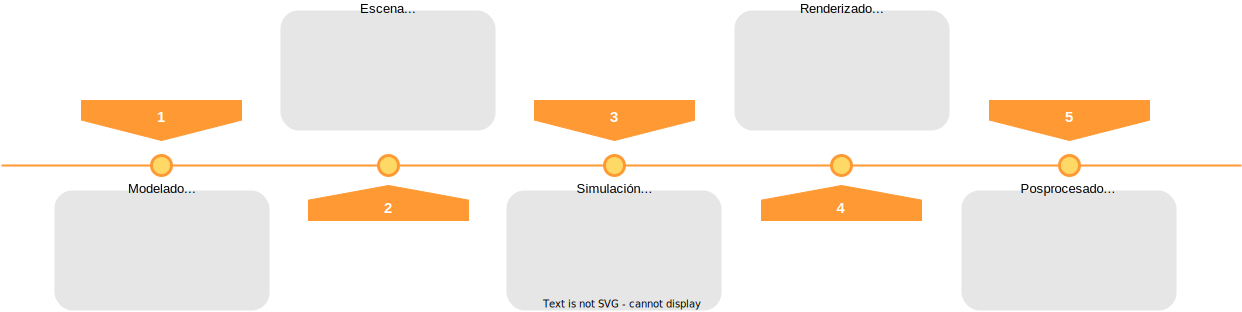
\includegraphics[width=0.9\textwidth]{Dataset/Arquitectura generador.pdf}
	\caption{Esquema de la arquitectura del generador de imágenes}
	\label{chap:Resumen fig:Arquitectura generador}
	\vspace{-5pt}
\end{figure}

Una vez desarrollado el \textit{dataset} necesario para llevar acabo este proyecto se puede introducir la solución desarrollada. Debido a la complejidad de la salida deseada (detección de la pieza y puntos de agarre) ha sido necesario desarrollar un sistema complejo compuesto por tres redes neuronales:

\begin{itemize}
\item \textit{YOLO}: se trata de la primera red neuronal empleada y desarrollada. Se encargará de detectar las piezas dentro de la zona de trabajo y se empleará como base para decidir que pieza se debe de recolectar. Es la única capa común a todas las piezas.

Con el fin de obtener los mejores resultados posibles se ha optado por emplear el proceso evolutivo de YOLO. Se trata de un proceso iterativo en el que en base a una función objetivo se van seleccionando los hiperparámetros de entrenamiento con el fin de optimizar el entrenamiento. Estos nuevos hiperparámetros se obtienen por medio de un algoritmo genético, de forma que los mejores resultados de la anterior iteración se emplearán como base para la creación de nuevos hiperparámetros. La función objetivo empleada se caracteriza por ser una combinación de $mAP@0.5$ con una contribución del 10\% y $mAP@0.5:0.95$ con una contribución del 90\%.

\begin{lstlisting}[language=Python]
 def fitness(x): 
     # Model fitness as a weighted combination of metrics 
     w = [0.0, 0.0, 0.1, 0.9]  # weights for [P, R, mAP@0.5, mAP@0.5:0.95] 
     return (x[:, :4] * w).sum(1) 
\end{lstlisting}

\item \textit{Tiny YOLO}: una red neuronal menor y menos potente pero con una mayor especialización. Esta red se encargará de determinar regiones con posibles puntos de agarre dentro de las piezas (previamente identificadas por \textit{YOLO}). Esta segunda capa es especifica para cada pieza y solo se aplicará a aquellas piezas de elevado volumen.

Esta segunda red neuronal se deberá de entrenar tantas veces como piezas de desee introducir al sistema. Es por ello que la carga computacional debe de ser reducida para evitar crear un sistema lento y poco eficiente. Por suerte, debido a la gran especialización de la red, solo debe de detectar regiones para un tipo de pieza, por ello se puede emplear la versión de YOLO de menor tamaño. La principal ventaja de YOLOv5 es el uso de recursos tanto a nivel computacional como de almacenamiento. La red ocupa 4 MB y cuenta con un total de 1.9 millones de neuronas. Pero a pesar de su reducido tamaño es capaz de lograr resultados sorprendentes capaces de competir con potentes y pesadas redes basadas en Fast-RCNN.

\item Regresor: se trata de la última capa del sistema de visión artificial. Se basa en la salida del \textit{Tiny YOLO} y determina para cada una de las posibles regiones de interés el punto de agarre óptimo y su vector normal. Esta última capa es especifica para cada pieza y solo se aplicará a aquellas piezas de elevado volumen.

El desarrollo de una red neuronal es un proceso laborioso que requiere de múltiples pruebas e intentos con el fin de conseguir desarrollar un sistema que aprenda y de forma optimizada. Es por ello por lo que se han tenido que desarrollar y entrenar múltiples redes para dar con un sistema óptimo. El primer paso en el desarrollo de la red ha sido comparar el impacto de diferentes tamaños de redes. Se han comparado redes con tres, cinco y siete capas convolucionales para determinar el número de capas necesarias para poder extraer las características. A continuación, se analiza el impacto del tamaño y profundidad de las redes \textit{fully connected}. A continuación, se comparan diferentes funciones de activación, diferentes criterios y optimizadores. Se observa en los resultados que la red sufre por sobreaprendizaje, es por ello que finalmente se implantan capas \textit{dropout}.
\end{itemize}

\begin{figure}[ht]
	\centering
	\includegraphics[width=0.5\textwidth]{Sistema de vision artificial/REGRESSION/CNNRegression.png}
	\caption{Estructura del regresor}
	\label{chap:Resumen fig:Estructura Regresor}
\end{figure}

\begin{figure}[ht]
	\centering
	\includegraphics[width=0.8\textwidth]{Sistema de vision artificial/Diagrama_vision.png}
	\caption{Esquema de la arquitectura del sistema de visión artificial}
	\label{chap:Resumen fig:Arquitectura sistema}
\end{figure}

\section*{3. Resultados}
Como se ha explicado anteriormente el sistema consta de dos elementos, el generador de imágenes y el sistema de visión artificial. Y a su vez estos son constituidos por múltiples módulos. Pero para poder analizar el comportamiento de estos se deben de analizar por separado y al conjunto.

El generador de imágenes debe de cumplir dos requisitos, los escenarios creados deben de ser aleatorios y las imágenes tienen que ser foto realistas. El segundo objetivo se consigue con creces gracias al uso de blender y a mapas de texturas de alta calidad. Por lo tanto nos debemos de fijar en mantener la aleatoriedad al crear las escenas. Para ello se han usado tres motores de aleatoriedad: numpy, random y uniformSO3 de Blenderproc. Y todos los motores son capaces de generar uniformidad aunque cabe destacar que uniformS03 se empleará para la generación de las posiciones y estas al emplear ángulos de euler se debe de emplear una distribución diferente.

\begin{figure}[ht]
	\ContinuedFloat
	\centering
	\begin{subfigure}[b]{0.3\linewidth}
		\includegraphics[width=\linewidth]{Dataset/Muestra_G1_a_sintetica.png}
	\end{subfigure}
	\begin{subfigure}[b]{0.3\linewidth}
		\includegraphics[width=\linewidth]{Dataset/Muestra_G3_sintetica.png}
	\end{subfigure}
	\begin{subfigure}[b]{0.3\linewidth}
		\includegraphics[width=\linewidth]{Dataset/Muestra_small_sintetica.png}
	\end{subfigure}
	\caption{Muestra de imágenes obtenidas mediante el generador de imágenes}
	\label{chap:Resumen fig:Muestras BlenderProc}
\end{figure}

\begin{figure}[ht]
	\ContinuedFloat
	\centering
	\begin{subfigure}[b]{0.3\linewidth}
		\includegraphics[width=\linewidth]{Dataset/numpy_uniform_histogram_1000.png}
	\end{subfigure}
	\begin{subfigure}[b]{0.3\linewidth}
		\includegraphics[width=\linewidth]{Dataset/random_choice_histogram_1000.png}
	\end{subfigure}
	\caption{Aleatoriedad de una distribución uniforme generada por NumPy y Random}
	\label{chap:Resumen fig:numpy and random uniform}
	
	\begin{subfigure}[b]{0.3\linewidth}
		\includegraphics[width=\linewidth]{Dataset/blenderproc_uniformS03_histogram_1.png}
	\end{subfigure}
	\begin{subfigure}[b]{0.3\linewidth}
		\includegraphics[width=\linewidth]{Dataset/blenderproc_uniformS03_histogram_2.png}
	\end{subfigure}
	\begin{subfigure}[b]{0.3\linewidth}
		\includegraphics[width=\linewidth]{Dataset/blenderproc_uniformS03_histogram_3.png}
	\end{subfigure}
	\caption{Aleatoriedad de \textit{uniformSO3} del paquete BlenderProc}
	\label{chap:Resumen fig:uniformS03}
\end{figure}

El segundo elemento que constituye el sistema es el conjunto de redes neuronales que componen el sistema de visión artificial. Como se ha explicado, esta compuesta por un total de tres redes y dependiendo del tipo de piezas se empleará una u todas las redes.

La primera red a entrenar es YOLO. Una vez completado el proceso evolutivo se han entrenado dos versiones de YOLO con diferentes hiperparámetros. En ambos casos se observa como la red neuronal es capaz de generalizar y extraer la información y características de las piezas. Pero también se observa la falta de entrenamiento ya que las métricas siguen mejorando cuando se detuvo el entrenamiento. Pero a pesar de ello se puede observar el gran rendimiento y capacidades de YOLO. También se observa una clara mejora al emplear los hiperparámetros obtenidos por el algoritmo evolutivo tanto en entrenamiento como en validación.

Por último, se ha obtenido la precisión y el \textit{recall} de validación (ver \autoref{chap:Sistema de visión artificial fig:YOLO Val PR}). Con la precisión se observa como con un nivel de confianza del 40\% se pueden obtener resultados con una precisión elevada. Y con \textit{recall} se observa como ha medida que aumentamos el nivel de confianza requerido aumenta el numero de falsos negativos (piezas no detectadas). Se han obtenido unos resultados prometedores (ver \autoref{chap:Sistema de visión artificial fig:YOLO Val Matrix}) caracterizados por una tasa de fallos reducida y una precisión elevada para niveles de confianza del 50\%. Los resultados son prometedores pero esto no implica que sean perfectos. La red presenta una clara ligera tendencia a dar falsos positivos a la hora de detectar algunas de las piezas.

\begin{figure}[H]
	\centering
    \includegraphics[width=0.45\textwidth]{Sistema de vision artificial/YOLO/Val/P_curve.png} \hfill
    \includegraphics[width=0.45\textwidth]{Sistema de vision artificial/YOLO/Val/R_curve.png}
	\caption{\textit{Precision y Recall} en validación de YOLO}
	\label{chap:Resumen fig:YOLO Val PR}
\end{figure}

La segunda red a entrenar es TINY YOLO. Tras entrenar durante un total de 250 \textit{epochs} se puede observar que la red neuronal ha conseguido aprender, extraer y generalizar la información disponible en el \textit{dataset}.Con lo que se ha podido reducir drásticamente las perdidas (\textit{object, class \& box}) tanto en entrenamiento como en validación. En este entrenamiento se puede apreciar que a pesar de ser un caso más simple, con un a red de menor tamaño y un mayor número de \textit{epochs}, la red todavía presenta un margen de mejora.

Tras finalizar el entrenamiento, se ha obtenido la precisión y el \textit{recall} en validación. Con la precisión se observa como con un nivel de confianza del 80\% se pueden obtener resultados con una precisión elevada y similares a la red YOLO con un nivel de confianza del 40\%. Esta reducción de precision frente a YOLO se puede deber a varios factores como el menor tamaño de red. El tipo de pieza a emplear, las regiones de interés no presentan bordes claramente definidos. O el tamaño de las piezas, debido al uso de Arucos de forma que todas las regiones son idénticas en tamaño y forma.

\begin{figure}[H]
	\centering
    \includegraphics[width=0.45\textwidth]{Sistema de vision artificial/TINY YOLO/Val/P_curve.png} \hfill
    \includegraphics[width=0.45\textwidth]{Sistema de vision artificial/TINY YOLO/Val/R_curve.png}
	\caption{\textit{Precision y Recall} en validación de TINY YOLO}
	\label{chap:Resumen fig:TINY YOLO Val PR}
\end{figure}

La última red a entrenar es el regresor. Esta tercera red neuronal se deberá de entrenar tantas veces como puntos de desee introducir al sistema. Es por ello que la carga computacional debe de ser reducida para evitar crear un sistema lento y poco eficiente. Teniendo esto en cuenta se ha desarrollado una red neuronal dividida en dos secciones, una primera sección basada en la convolución y encargada de extraer las características de la pieza. Y una segunda sección del tipo \textit{fully connected} basada en perceptrones que se encargarán de estimar las coordenadas y el vector normal del punto de agarre.

Destaca con los mejores resultados la red con el mayor número de capas de convolución y sin capas \textit{Dropout}. Y con este tipo de red se consigue obtener un error entorno al 5\% en validación para los vectores normales y entorno al 1-2\% para la determinación del punto de agarre. También destaca en esta red los errores de validación de los vectores normales donde a pesar del entrenamiento se dan situaciones en donde los resultados obtenidos empeoran al aumentar el entrenamiento. Esto se debe a una combinación de sobreaprendizaje junto un la utilización de un \textit{dataset} sesgado. Esto conlleva a la red a asumir las posiciones de los vectores normales y es por ello por lo que aumenta el error total a pesar del entrenamiento.

\begin{figure}[ht]
\centering
\begin{tabular}{cc}
\includegraphics[width=0.6\textwidth]{Sistema de vision artificial/REGRESSION/val_loss.png} &
\includegraphics[width=0.2\textwidth]{Sistema de vision artificial/REGRESSION/legend.png}
\end{tabular}
\caption{Comparativa de las fases de validación del regresor}
\label{chap:Resumen fig:Validación Regresor}
\end{figure}

\section*{4. Conclusiones}
El desarrollo de este proyecto se caracteriza por cumplir dos grandes objetivos/metas. En primer lugar, su desarrollo ha permitido la creación de un sistema basado en redes neuronales capaz de identificar piezas y sus puntos de agarre óptimos. Y en segundo lugar ha permitido comprobar las capacidades de aprendizaje de una red neuronal al emplear un \textit{dataset} sintético. Es por ello que se debe de analizar el sistema desde las dos perspectivas.

Para el desarrollo del sistema de identificación de puntos de agarre se ha tenido que desarrollar un \textit{dataset} sintético que refleje la realidad y permita aumentar el número de imágenes para el entrenamiento. Durante el desarrollo de este sistema se presto especial atención en representar lo mejor posible la realidad y el entorno de trabajo. De esta forma varios de los escenarios y de las configuraciones usadas se limitan a representar los escenarios observados en la planta de ensamblaje. Esta decisión desgraciadamente ha conllevado la generación de un \textit{dataset} sesgado en donde la mayoría de las piezas se encuentran en una posición predefinida por el escenario. Es por ello por lo que se recomienda mejorar la aleatoriedad del sistema introduciendo mas escenarios que a pesar de que no reflejen la realidad si permitan la obtención de imágenes con mayor riqueza y eviten el sesgado del la red.

El nuevo sistema de visión artificial ha conseguido obtener el punto de agarre óptimo para las piezas grandes y se ha asumido el centro de las piezas pequeñas como un buen punto de agarre. En base a los resultados obtenidos en la fase de validación, el sistema se muestra capaz con errores pequeños y pocos \textit{outliers}. Desgraciadamente el comportamiento de las redes solo se ha podido analizar frente a un \textit{dataset} sintético pero no frente a una situación real. Para determinar con precisión el alcance y la capacidad del sistema se requiere de un \textit{dataset} real.

Pero esta falta de un \textit{dataset} real no impide que se pueda analizar la estructura del sistema y se planteen puntos de mejora. La red presenta grandes puntos fuertes como su modularidad. La cual permite la inclusión de nuevas piezas sin afectar al rendimiento de las ya implementadas y sin la necesidad de entrenar toda la red frente a un \textit{dataset} con todas las piezas. Esto mejora los resultados a la vez que se reduce el tiempo de entrenamiento para nuevas piezas. Por el contrario, esta modularidad implica una perdida de eficiencia al tener que analizar múltiples veces una misma escena. Se plantea a futuro la posibilidad de desarrollar una única red que a su vez presente un formato modular para adaptarse a cada pieza. Pero al tratarse de una sola red se podrá realizar todo el proceso con un solo análisis.  
}